\documentclass{article}
\usepackage[utf8]{inputenc}
\usepackage{geometry}
\usepackage{titling}
\usepackage{graphicx}


\geometry{a4paper, total={170mm,257mm}, left=20mm, top=20mm}

\title{\Huge Data Exploration Project}
\author{Timo Nössler}
\date{\vspace{2cm}05.03.2024}

\begin{document}
\clearpage\maketitle
\thispagestyle{empty}
\begin{center}
\textbf{Matrikelnummer:} 123456789
\end{center}
\newpage
\tableofcontents
\newpage


\section{Einleitung}
\subsection{Vorstellung Datensatz}
Dieser Datensatz enthält Informationen über verschiedene Attribute einer Reihe von Äpfeln, die Aufschluss über deren Eigenschaften geben. Es sind Details wie eine eindeutige Frucht-ID, Größe, Gewicht, Süße, Knackigkeit, Saftigkeit, Reifegrad, Säuregehalt und Qualität. 
\begin{table}[h]
\centering
\begin{tabular}{|c|c|}
\hline
\textbf{Attribut} & \textbf{Beschreibung} \\
\hline
A\_id & Unique identifier for each fruit \\
Size & Size of the fruit \\
Weight & Weight of the fruit \\
Sweetness & Degree of sweetness of the fruit \\
Crunchiness & Texture indicating the crunchiness of the fruit \\
Juiciness & Level of juiciness of the fruit \\
Ripeness & Stage of ripeness of the fruit \\
Acidity & Acidity level of the fruit \\
Quality & Overall quality of the fruit \\
\hline
\end{tabular}
\caption{Attributes of the fruit table}
\end{table}


\subsection{Erklärung der Referenzwerte}
Die Hintergrundrecherche zu dem Datensatz hat ergeben, dass sich die Daten auf einen Standard Apfel beziehen und somit keine Werte in einer SI Einheit darstellen. Nach dem Bundeszentrum für Ernährung muss ein Apfel in Europa eine Mindestgröße von 60 Milimeter im Durchmesser aufweisen und ein Mindestgewicht von 90 Gramm haben. Somit wird bei einem Wert von über Null von einem über dem Standard liegenden Apfel ausgegangen und bei einem Wert unter Null somit von einem Apfel unter den Standard Maßen. Da die Daten aus den Vereinigten Staaten von Amerika stammen werden im folgenden beispielhaft die Standard Apfelmaße der USA aufegführt (Figure 1).
\begin{figure}[h]
\centering
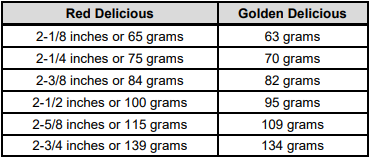
\includegraphics[scale=.8]{"../images/AppleStandard.png"}
\caption{Bsp. Apfelstandard USA}
\label{fig:meine-grafik}
\end{figure}


\section{Daten Exploration}


\subsection{Technische Datenanalyse}
Die Charakterisierung der Daten erfolgt auf der Grundlage verschiedener statistischer und erläuternden Funktionen die auf den Datensatz angewendet werden. Dies dient dazu einen umfassenden Einblick in den Datensatz zu erhalten. Der "Overall Overview" ermöglicht einen ersten Überblick über die Daten. Ergänzt wird der Einblick durch die "Data Summary. Hier werden Informationen über die Dimension des Datensatzes gewonnen.Die "Data Info" gibt detaillierte Informationen über die Art der Daten in jeder Spalte, einschließlich der Anzahl der Nicht-Null-Einträge. Dies hilft, die Art der Daten zu verstehen und mögliche Probleme der Datenqualität, wie fehlende Werte zu identifizieren. Die "Data Description" liefert statistische Kennzahlen zu den numerischen Spalten des Datensatzes, wie zum Beispiel den Mittelwert, die Standardabweichung und Quartile. Dies hilft, ein besseres Verständnis für die
Verteilung der Daten zu entwickeln. Zuletzt zeigt die Auswertung der "Missing Values" die Anzahl der fehlenden Werte in jeder Spalte des Datensatzes. Dies ist entscheidend, um potenzielle Datenqualitätsprobleme zu identifizieren und zu entscheiden, wie mit den fehlenden Werten umgegangen werden soll. Insgesamt bietet die Datenexploration einen fundierten Überblick über den vorliegenden Datensatz und dient als Grundlage zur weiteren Verarbeitung.\\
!!HIER KOMMEN NOCH TABELLEN ZU DEN AUSWERTUNGEN!!

\subsection{Visuelle Datenanalyse}
Die Visualisierungen werden verwendet, um die Beziehung zwischen verschiedenen Attributen von Äpfeln und deren Gesamtqualität zu untersuchen.\\ 
Der Boxplot zeigt die Verteilung der spezifischen Attribute (Größe, Gewicht, Süße, Knackigkeit, Saftigkeit, Reife, Säure) in Bezug auf die Qualität der Äpfel. So wird ermöglicht einen Eindruck über die Verteilung und die Ausreißer in den Attributen in Abhängigkeit von der Qualität zu visualisieren.\\
Die Berechnung der Summe der "guten" und "schlechten" Werte sowie die anschließende Darstellung als Kreisdiagramm ermöglicht es, die prozentuale Verteilung von guten und schlechten Äpfeln, in dem Datensatz darzustellen. Die Erstellung einer Heatmap in Verbindung mit einer Korrelationsmatrix gibt einen Überblick über mögliche Korrelationen zwischen den verschiedenen Attributen. Es wird gezeigt, wie stark, oder schwach, die Attribute untereinander korrelieren. Des weiteren ermöglicht es, Muster und Zusammenhänge zu identifizieren.\\ Abschließend visualisiert der Pairplot die Beziehung zwischen den verschiedenen Merkmalen der Äpfel durch Streudiagramme und Histogramme. Durch die Farbcodierung nach Qualität können Unterschiede und Muster zwischen guten und schlechten Äpfeln identifiziert werden. Insgesamt ermöglichen diese Schritte eine umfassende Analyse der Attribute in Bezug auf die Qualität und tragen dazu bei, Muster, Zusammenhänge und Unterschiede zwischen guten und schlechten Äpfeln zu identifizieren.\\
!! HIER KOMMEN NOCH AUSGEWÄHLTE VISUALISIERUNGEN!!

\subsection{Feature Engineering}
Ein Decision Tree Classifier ist ein Werkzeug im Bereich des maschinellen Lernens, das zur Klassifizierung von Daten verwendet wird. Es basiert auf dem Prinzip der rekursiven Partitionierung, bei der der Datensatz in immer kleinere Teilmengen aufgeteilt wird, um Entscheidungsregeln abzuleiten.\\ 
Die Überprüfung der Wichtigkeit einzelner Werte mittels eines Decision Tree Classifiers ermöglicht es, die Beiträge der verschiedenen Merkmale zur Klassifikation zu verstehen und diejenigen Merkmale zu identifizieren, die entscheidend für die Klassifikation sind. Dies wiederum kann dazu beitragen, die Modellinterpretation zu verbessern, die Merkmalsauswahl zu optimieren und Einblicke in die zugrunde liegenden Daten zu gewinnen. Die Auswertung des Decision Tree Classifier ergibt, dass die 'Size' (22\%), 'Ripeness' (20\%), 'Juiciness' (19\%) den größten Einfluss auf die Klassifiezierung der Äpfel haben. 
\begin{table}[h]
\centering
\begin{tabular}{|c|c|}
\hline
\textbf{Attribut} & \textbf{Beschreibung} \\
\hline
Size & 22\% \\
Weight & 11\% \\
Sweetness & 13\% \\
Crunchiness & 1\% \\
Juiciness & 19\% \\
Ripeness & 20\% \\
Acidity & 13\% \\
\hline
\end{tabular}
\caption{Einfluss der Attribute}
\end{table}

\subsection{Datensatz Split}
Dieser Prozess wird als Datenpartitionierung bezeichnet und ist wichtig, um sicherzustellen, dass das Modell angemessen trainiert, validiert und getestet wird, ohne dass die Ergebnisse durch Overfitting oder Underfitting beeinflusst werden. Durch diese Aufteilung des Datensatzes in Trainings-, Validierungs- und Testsets können Modelle zunächst auf den Trainingsdaten trainiert und dann auf den Validierungsdaten optimiert werden. Anschließend kann die Leistung des Modells mit den Testdaten bewertet werden, um sicherzustellen,  dass es auf neuen, unabhängigen Daten gut generalisiert.

\subsection{Auswahl der Metriken}
Angesichts der Tatsache, dass ein Apfelhändler Gefahr läuft, seinen Ruf zu schädigen, wenn er überreife Äpfel an seine Kunden verkauft, ist es entscheidend, dass das Klassifizierungsmodell in erster Linie den Recall optimiert. Der Recall misst den Anteil der tatsächlich positiven Fälle, die korrekt als solche identifiziert wurden. In diesem Szenario ist es wichtiger, sicherzustellen, dass überreife oderminderwertige Äpfel als solche erkannt und aussortiert werden, selbst wenn dies bedeutet, dass gelegentlich ein qualitativ hochwertiger Apfel fälschlicherweise aussortiert wird. Der wirtschaftliche Schaden, der durch den Verlust eines guten Apfels entsteht, wird als geringer angesehen als der Schaden, der entsteht, wenn minderwertige Äpfel an den Einzelhandel weitergegeben werden und so das Vertrauen der Kunden beeinträchtigen.\\
Das Optimieren auf Recall bedeutet, dass das Modell so eingestellt wird, dass es möglichst wenige minderwertige Äpfel als qualitativ hochwertig klassifiziert. Dies kann durch die Anpassung der Entscheidungsgrenze des Modells erreicht werden, wodurch die Klassifizierungsschwelle verschoben wird, um den Fokus auf die Identifizierung von minderwertigen Äpfeln zu legen, selbst wenn dadurch gelegentlich gute Äpfel fälschlicherweise aussortiert werden.\\
Durch diese Schwerpunktsetzung auf den Recall wird sichergestellt, dass das Modell seine Fähigkeit verbessert, minderwertige Äpfel zuverlässig zu erkennen, was letztendlich dazu beiträgt, den Ruf des Apfelhändlers zu schützen und den wirtschaftlichen Schaden zu minimieren.


\section{Maschinelles Lernen}

\subsection{Auswahl und Beschreibung der Methode}
In dieser Arbeit wir ein Gradient Boost Algorithmus verwendet. Gradient Boosting ist eine Methode des maschinellen Lernens, die zur Lösung von Klassifikations- und Regressionsproblemen eingesetzt wird. Sie funktioniert durch das schrittweise Hinzufügen von Modellen, um die Vorhersagegenauigkeit zu verbessern. Im Gegensatz zu Random Forests werden die Modelle bei Gradient Boosting nacheinander erstellt, anstatt parallel.\\
Der Prozess beginnt mit der Erstellung eines einfachen Modells (normalerweise ein Entscheidungsbaum) aus den Trainingsdaten. Anschließend werden Vorhersagen auf den Trainingsdaten getroffen und mit den tatsächlichen Werten verglichen. Eventuelle Fehler werden berechnet und mit einem weiteren Modell korrigiert. Dieser Vorgang wiederholt sich, indem jedes Modell die Fehler des vorherigen Modells korrigiert und somit die Vorhersagegenauigkeit insgesamt verbessert.\\
Der Gradient Boosting-Algorithmus verwendet das Gradientenverfahren, um Fehler zu ermitteln und zu minimieren. Hierbei werden Fehler in Form von Gradienten bewertet und das nächste Modell wird genutzt, um den Gradienten in die entgegengesetzte Richtung zu "boosten" (d.h. zu minimieren).\\
Gradient Boosting hat den Vorteil, tiefe und komplexe Modelle zu erstellen, die in der Lage sind, sehr kleine Unterschiede in den Daten zu erkennen. Es wurde gezeigt, dass Gradient Boosting in vielen Anwendungen eine höhere Leistung als Random Forest oder andere Methoden bietet.\\
Es gibt verschiedene Implementierungen von Gradient Boosting, darunter XGBoost und LightGBM, die zu den bekanntesten gehören. In dieser Arbeit wird der XGBoost Algorithmus verwendet.\\
Allerdings hat Gradient Boosting auch Nachteile. Eine Herausforderung bei dieser Methode ist, dass sie mehr Zeit und Speicher benötigt als manche Alternativen, da jedes Modell in der Sequenz erstellt werden muss. Außerdem ist es schwierig, die passenden Parameter zur Optimierung des Modells auszuwählen. Jedoch überwiegen in diesem Fall die Vorteile wie Skalierbarkeit, Regulierung und die Flexibilität. So kann der Algorithmus auch auf große Datenmengen angewandt werden, er bietet verschiedene Möglichkeiten um Over-, und Underfitting zu vermeiden. Auch die Flexibilität zwischen unterschiedlichen Datentypen und nicht vorhandene Daten ist ein Vorteil des XGBoost.


\end{document}